\documentclass[conference]{IEEEtran}
\IEEEoverridecommandlockouts
\usepackage{cite}
\usepackage{amsmath,amssymb,amsfonts}
\usepackage{algorithm}
\usepackage{algorithmic}
\usepackage{graphicx}
\usepackage{textcomp}
\usepackage{xcolor}
\usepackage{booktabs}
\usepackage{tikz}
\usetikzlibrary{arrows.meta,positioning,fit,calc}
\usepackage[hidelinks]{hyperref}
\graphicspath{{../figures/}}
\hypersetup{pdfauthor={Deepankar},pdftitle={Beyond Development: Explaining Climate Resilience Across Indian Districts}}

\makeatletter
\newcommand{\linebreakand}{%
  \end{@IEEEauthorhalign}
  \hfill\mbox{}\par
  \mbox{}\hfill\begin{@IEEEauthorhalign}
}
\makeatother

% compact "where" list of the symbols under each equation
\newenvironment{symlist}{\par\vspace{-2pt}\noindent\footnotesize where:\par\begin{list}{}{\setlength{\leftmargin}{4.4em}\setlength{\labelwidth}{4.1em}\setlength{\labelsep}{0.3em}\setlength{\itemsep}{0pt}\setlength{\parsep}{0pt}\setlength{\topsep}{1pt}\renewcommand{\makelabel}[1]{##1\hfil}}}{\end{list}\vspace{2pt}}

\begin{document}

\title{Beyond Development: Explaining Climate Resilience Across Indian Districts with a Hadoop Pipeline and a Boosted Attentive Climate Push Network}

\author{
\IEEEauthorblockN{\textbf{Sehjodh Grewal}}
\IEEEauthorblockA{Department of Networking and Communications,\\
School of Computing,\\
SRM Institute of Science and Technology,\\
Kattankulathur, Chengalpattu -- 603203, TN, India.\\
sg2827@srmist.edu.in}
\and
\IEEEauthorblockN{\textbf{Devanshu Kumar}}
\IEEEauthorblockA{Department of Networking and Communications,\\
School of Computing,\\
SRM Institute of Science and Technology,\\
Kattankulathur, Chengalpattu -- 603203, TN, India.\\
dk5504@srmist.edu.in}
\linebreakand
\IEEEauthorblockN{\textbf{Deepankar}}
\IEEEauthorblockA{Department of Networking and Communications,\\
School of Computing,\\
SRM Institute of Science and Technology,\\
Kattankulathur, Chengalpattu -- 603203, TN, India.\\
dz9629@srmist.edu.in}
\and
\IEEEauthorblockN{\textbf{Tanmay Singh}}
\IEEEauthorblockA{Department of Networking and Communications,\\
School of Computing,\\
SRM Institute of Science and Technology,\\
Kattankulathur, Chengalpattu -- 603203, TN, India.\\
ts4494@srmist.edu.in}
\linebreakand
\IEEEauthorblockN{\textbf{Dr. Banu Priya Prathaban*}}
\IEEEauthorblockA{Department of Networking and Communications, School of Computing\\
SRM Institute of Science \& Technology\\
Kattankulathur, Chennai, India -- 603203.\\
banuprip2@srmist.edu.in\\
\textit{Corresponding Author}}
}

\maketitle

\begin{abstract}
Development indicators are often used as a shorthand for how well an Indian district can cope with climate stress, yet many developed districts remain highly vulnerable while some poorer ones are resilient. We study this gap for 469 districts in 21 states by combining the 2021 district climate vulnerability index, Census 2011 development variables and 30 years (1991--2020) of daily India Meteorological Department (IMD) rainfall and temperature grids, about 212 million gridded values. A single-node Hadoop pipeline stores the data in HDFS (1.08 GB), turns 7,013,120 district-day rows into 19,200 district-year climate indices with MapReduce on YARN, builds the 30-year baseline and the analysis table with Hive, and groups districts into climate regimes with Spark. On this table we propose B-ACPN, a Boosted Attentive Climate Push Network: a random-forest stage supplies a first risk score, and a small neural network adds a development term and a development-gated, attention-weighted \emph{climate push}, averaged over five networks, with Monte Carlo Dropout and conformal uncertainty. On 25 repeated cross-validation folds B-ACPN reaches a ROC-AUC of 0.820, accuracy 0.738 and F1 0.728, the highest of six models; it is significantly better than random forest, a standard MLP, a linear SVM and logistic regression, and comparable to gradient-boosted trees (p = 0.55). Its climate push separates the anomalous districts from the expected ones (p $<$ 0.001), showing that climate, not only development, explains why developed districts can stay vulnerable.
\end{abstract}

\begin{IEEEkeywords}
climate vulnerability, India, Hadoop, MapReduce, Hive, Spark, deep learning, explainable machine learning, conformal prediction
\end{IEEEkeywords}

\section{Introduction}
India is among the countries most exposed to heavy rainfall, droughts and heat, and district administrations are the level at which adaptation is planned. National assessments rank districts by climate vulnerability \cite{ceew2021,dst2020}, and a common assumption is that more developed districts, with higher literacy and less dependence on farming, are less vulnerable. The data only partly agree. In our sample development explains just 13\% of the variation in the vulnerability index ($R^2$ = 0.127), and 181 of 469 districts (38.6\%) break the expected pattern: they are developed yet vulnerable, or less developed yet resilient.

Explaining these anomalies needs long, fine-grained climate records. Thirty years of daily IMD grids \cite{pai2014,srivastava2009} for the whole country are too large to handle comfortably as plain files, and the same steps (aggregating days into years, years into a baseline, and joining with development data) recur whenever the period or the variables change. We therefore built the processing as a Hadoop pipeline. On the modelling side, an ordinary classifier says whether a district is highly vulnerable but not \emph{why}. We wanted a model that is accurate and that also separates the climate contribution from the development contribution for every district.

The main contributions of this work are:
\begin{itemize}
\item A reproducible Big Data pipeline in which HDFS, MapReduce on YARN, Hive and Spark each do a measured job, with every step checked against an independent implementation.
\item A preprocessing workflow without imputation, evaluated with eight error metrics, including the error that a naive nearest-cell aggregation would have introduced.
\item B-ACPN, a hybrid model that boosts a random-forest score with a development-gated attentive climate network and gives a per-district climate push with uncertainty.
\item A fair comparison with five existing models on identical folds, with 17 metrics, confidence intervals, corrected significance tests, an ablation study and a before/after analysis of preprocessing.
\end{itemize}

The rest of the paper is organised as follows. Section~II reviews related work. Section~III describes the data, the preprocessing and the Big Data pipeline. Section~IV presents B-ACPN. Section~V reports the experiments, and Section~VI discusses limitations before Section~VII concludes.

\section{Related Work}
\subsection{Climate vulnerability in India}
Mohanty and Wadhawan \cite{ceew2021} mapped district-level exposure and vulnerability to hydro-meteorological extremes across India, and the Department of Science and Technology \cite{dst2020} published a common framework for district vulnerability assessment. The IPCC \cite{ipcc2022} stresses that vulnerability depends on both exposure and adaptive capacity. These assessments build composite indices; they do not ask why districts with similar development end up with different vulnerability, which is our focus.

\subsection{Big Data platforms}
HDFS \cite{shvachko2010} stores large files as replicated blocks, MapReduce \cite{dean2008} expresses batch aggregations as map and reduce functions, and YARN \cite{vavilapalli2013} schedules them. Hive \cite{thusoo2009} adds SQL over HDFS, and Spark \cite{zaharia2016} keeps data in memory, which suits iterative algorithms; its MLlib library \cite{meng2016} provides standard classifiers. We use each tool for the step it fits best rather than forcing all steps into one engine.

\subsection{Learning on tabular data}
For small tabular datasets, tree ensembles such as random forests \cite{breiman2001} and gradient boosting \cite{friedman2001} remain strong, and Grinsztajn et al. \cite{grinsztajn2022} showed that they still often beat deep networks. Attention over input features, as in TabNet \cite{arik2021}, makes a network's use of features visible. Stacking \cite{wolpert1992} feeds one model's out-of-fold predictions to another. B-ACPN combines these ideas: the trees provide accuracy, and the network adds a structured, explainable correction.

\subsection{Uncertainty}
Monte Carlo Dropout \cite{gal2016} approximates Bayesian uncertainty by keeping dropout active at prediction time, and split conformal prediction \cite{angelopoulos2021} turns any classifier's scores into prediction sets with a coverage guarantee. Both are cheap and fit our small model.

\section{Data and Big Data Pipeline}
\subsection{Sources}
Table~\ref{tab:data} lists the sources. The outcome is the 2021 district climate vulnerability index from NITI Aayog's National Data and Analytics Platform (NDAP, dataset 7160), split at its median into High and Low vulnerability. Five development variables come from Census 2011 (literacy, female literacy, agricultural-worker share) and NDAP (MGNREGA days, yield variability). Eight climate hazard variables are computed from the IMD grids. The index is only the target and is never an input.

\begin{table}[t]
\centering
\caption{Data sources}
\label{tab:data}
\scriptsize
\setlength{\tabcolsep}{3.5pt}
\begin{tabular}{lcccc}
\toprule
Dataset & Source & Year & Size & Role \\
\midrule
Vulnerability index & NDAP 7160 & 2021 & 699$\times$79 & target, 2 dev. \\
Census abstract & Census & 2011 & 640 dist. & 3 dev. \\
Daily rainfall, 0.25\textdegree{} & IMD & 1991--2020 & 763 MB & hazards \\
Daily Tmax/Tmin, 1\textdegree{} & IMD & 1991--2020 & 84 MB & hazards \\
Boundaries & DataMeet & 2011 & 641 polygons & weights \\
\bottomrule
\end{tabular}
\end{table}

\subsection{Preprocessing}
Census counts were converted to rates and checked against national totals: the population matches the official figure exactly and national literacy differs by 0.0019 percentage points. NDAP and Census districts were matched inside state clusters (Andhra Pradesh with Telangana, Jammu and Kashmir with Ladakh) by exact name, an alias table and fuzzy matching; 602 of 699 NDAP districts were matched with no duplicate codes, and two wrong fuzzy matches were found by hand and blocked. NDAP is sparse (75\% of all cells empty), so we kept only the five development variables that are well covered and dropped districts with missing values instead of imputing them, leaving 469 complete districts.

Grid values were turned into district values with area weights. The weight of grid cell $c$ for district $d$ is
\par\noindent\begin{minipage}{\columnwidth}
\begin{equation}
w_{c,d} = \frac{A(c \cap d)\cos\varphi_c}{\sum_{c'} A(c' \cap d)\cos\varphi_{c'}},
\end{equation}
\begin{symlist}
\item[$w_{c,d}$] area weight of grid cell $c$ for district $d$;
\item[$A(c \cap d)$] share of cell $c$ lying inside district $d$, computed in an equal-area projection;
\item[$\varphi_c$] latitude of the centre of cell $c$ (cells shrink towards the north);
\item[$c'$] any grid cell overlapping district $d$; the sum makes the weights add up to one.
\end{symlist}
\end{minipage}\par

The weights of every district sum to one within $10^{-7}$. Daily district values are weighted means over the cells with data that day; IMD missing codes stay missing and are never set to zero. An automatic check confirms the grid orientation: Chennai's rainfall must peak in the north-east monsoon (October--December). The result is a table of 7,013,120 district-day rows.

Table~\ref{tab:prep} evaluates the two preprocessing steps that have an exact reference with eight error metrics. Replacing our area-weighted rainfall by the naive nearest-cell value would cause an RMSE of 287 mm and a MAPE of 11.1\% per district; the MapReduce indices agree with an independent pandas recomputation to rounding error.

\begin{table}[t]
\centering
\caption{Preprocessing error metrics}
\label{tab:prep}
\footnotesize
\setlength{\tabcolsep}{3.5pt}
\begin{tabular}{lcc}
\toprule
Metric & Nearest cell vs ours (mm) & MapReduce vs pandas$^{*}$ \\
\midrule
RMSE & 286.9 & 0.003 \\
MSE & $8.2\times10^{4}$ & $8.4\times10^{-6}$ \\
MAE & 151.7 & 0.003 \\
MAPE & 11.08\% & 0.008\% \\
$R^2$ & 0.904 & 0.999999 \\
NRMSE & 0.034 & $1.9\times10^{-4}$ \\
MedAE & 87.0 & 0.002 \\
Bias (ME) & 5.045 & $-2.2\times10^{-5}$ \\
\bottomrule
\end{tabular}
\\[2pt]\parbox{0.95\columnwidth}{\scriptsize Left: annual rainfall of 636 districts, 2020; reference = our area-weighted value. $^{*}$Worst of the seven indices over 19,200 district-years.}
\end{table}

\subsection{Big Data pipeline}
Fig.~\ref{fig:pipe} shows the pipeline. It runs on a single-node, pseudo-distributed Hadoop 3.3.6 cluster (HDFS replication 1, 128 MB blocks, 2 vCPU, 12.7 GB RAM) in Google Colab, with Java 8, Hive 3.1.3 and Spark 3.5.3. Colab has no SSH, so each daemon is started directly. Because the cluster has one node we make no claim about multi-machine speed-up.

\begin{figure}[t]
\centering
\resizebox{\columnwidth}{!}{%
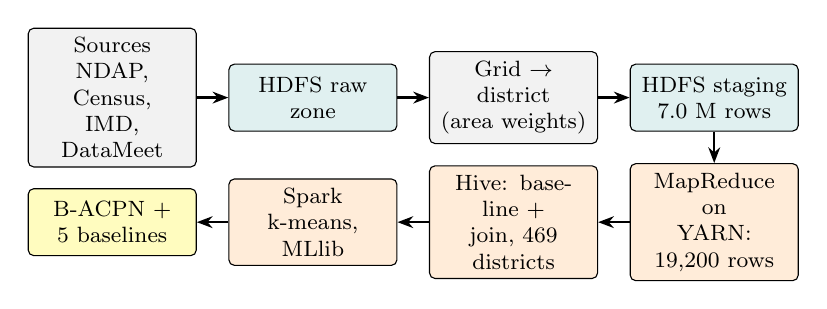
\begin{tikzpicture}[node distance=4mm and 4mm,
  box/.style={draw, rounded corners=2pt, align=center, font=\footnotesize, minimum height=8.5mm, text width=19mm, fill=#1},
  box/.default=white, arr/.style={-{Stealth[length=2mm]}, thick}]
\node[box=gray!10] (src) {Sources\\NDAP, Census,\\IMD, DataMeet};
\node[box=teal!12, right=of src] (raw) {HDFS raw\\zone};
\node[box=gray!10, right=of raw] (grid) {Grid $\rightarrow$ district\\(area weights)};
\node[box=teal!12, right=of grid] (stg) {HDFS staging\\7.0 M rows};
\node[box=orange!15, below=of stg] (mr) {MapReduce on\\YARN: 19,200 rows};
\node[box=orange!15, left=of mr] (hive) {Hive: baseline +\\join, 469 districts};
\node[box=orange!15, left=of hive] (spark) {Spark\\k-means, MLlib};
\node[box=yellow!25, left=of spark] (model) {B-ACPN +\\5 baselines};
\draw[arr] (src) -- (raw); \draw[arr] (raw) -- (grid); \draw[arr] (grid) -- (stg); \draw[arr] (stg) -- (mr);
\draw[arr] (mr) -- (hive); \draw[arr] (hive) -- (spark);
\draw[arr] (spark) -- (model);
\end{tikzpicture}}
\caption{Processing pipeline. Teal: HDFS storage zones; orange: Big Data processing; yellow: models.}
\label{fig:pipe}
\end{figure}

HDFS holds three zones: \emph{raw} for the untouched sources, \emph{staging} for the district-day table and \emph{processed} for job outputs. MapReduce, run with Hadoop Streaming, keys every district-day row by (district, year); each reducer sorts the days of one district-year by date and computes seven indices: annual rainfall, heavy-rain days (rain $\ge$ 64.5 mm), maximum five-day rainfall, longest dry spell (rain $<$ 1 mm), mean daily maximum temperature, hot days ($T_{\max} \ge$ 35\,\textdegree C) and tropical nights ($T_{\min} \ge$ 25\,\textdegree C). Incomplete years are left blank rather than set to zero. Hive then averages each index over 1991--2020, adds the inter-annual standard deviation of rainfall as rain variability, and joins the result with the development table on the Census district code. Spark k-means on the eight standardised hazard variables, with $k$ chosen by the silhouette score \cite{rousseeuw1987}, groups districts into climate regimes. Table~\ref{tab:bigdata} summarises the jobs.

\begin{table}[t]
\centering
\caption{Big Data jobs (single node, Colab run)}
\label{tab:bigdata}
\footnotesize
\setlength{\tabcolsep}{3.5pt}
\begin{tabular}{lccc}
\toprule
Job & Input & Output & Result \\
\midrule
HDFS load & raw + staging & 3 zones & 1.08 GB \\
MapReduce & 7,013,120 rows & 19,200 rows & 333 s \\
Hive & 19,200 rows + dev. & 469 districts & = pandas \\
Spark k-means & 8 hazards & 2 regimes & silh. 0.651 \\
\bottomrule
\end{tabular}
\end{table}

\section{Proposed Model: B-ACPN}
\subsection{Overview}
Let $\mathbf{x}_i = (\mathbf{d}_i, \mathbf{h}_i)$ be the five development and eight hazard variables of district $i$ and $y_i \in \{0,1\}$ its vulnerability class. B-ACPN (Fig.~\ref{fig:model}) has three parts.

\emph{Tree stage.} A random forest \cite{breiman2001} with 500 trees and a minimum leaf size of two is trained on all 13 features. For training districts its probability is computed out-of-fold over five inner folds, so the next stage never sees a score that the forest produced on its own training rows. The tree score is the log-odds
\par\noindent\begin{minipage}{\columnwidth}
\begin{equation}
s_i = \log\frac{\hat p^{\,\text{RF}}_i}{1-\hat p^{\,\text{RF}}_i}.
\end{equation}
\begin{symlist}
\item[$s_i$] tree score (log-odds) of district $i$;
\item[$\hat p^{\,\text{RF}}_i$] random-forest probability that district $i$ is highly vulnerable (out-of-fold for training districts).
\end{symlist}
\end{minipage}\par


\emph{Deep stage.} A small network starts from $s_i$ and adds a development term and a climate push:
\par\noindent\begin{minipage}{\columnwidth}
\begin{align}
b_i &= s_i + \mathbf{w}^{\top}\mathbf{d}_i + \beta, \\
\mathbf{a}_i &= \operatorname{softmax}\!\big(W_2 \tanh(W_1 \mathbf{h}_i)\big),\quad \tilde{\mathbf{h}}_i = 8\,\mathbf{a}_i \odot \mathbf{h}_i, \\
c_i &= f_\theta(\tilde{\mathbf{h}}_i)\cdot 2\,\sigma\!\big(g_\phi(\mathbf{d}_i)\big).
\end{align}
\begin{symlist}
\item[$b_i$] baseline logit of district $i$ (tree score plus development term);
\item[$\mathbf{d}_i$] the five standardised development features of district $i$;
\item[$\mathbf{w}, \beta$] learned weights and bias of the development term;
\item[$\mathbf{h}_i$] the eight standardised climate-hazard features of district $i$;
\item[$W_1, W_2$] learned weight matrices of the attention network;
\item[$\mathbf{a}_i$] attention weights over the eight hazards (they sum to one);
\item[$\tilde{\mathbf{h}}_i$] attention-weighted hazards (the factor 8 keeps the mean weight at one);
\item[$\odot$] element-wise product;
\item[$c_i$] climate push of district $i$ ($>0$: climate adds risk, $<0$: climate protects);
\item[$f_\theta$] climate network (MLP with a residual block) with parameters $\theta$;
\item[$g_\phi$] development-gate network with parameters $\phi$;
\item[$\sigma$] sigmoid function, $\sigma(x) = 1/(1+e^{-x})$.
\end{symlist}
\end{minipage}\par

Here $\mathbf{a}_i$ are attention weights over the hazards, $f_\theta$ is a linear layer (8$\rightarrow$16) with ReLU and dropout 0.3, a residual block \cite{he2016} (linear, batch normalisation, ReLU, dropout, skip connection) and a bias-free output layer, and the development gate $2\sigma(g_\phi)$, with $g_\phi$ a 5$\rightarrow$4$\rightarrow$1 tanh network, scales the push between 0 and 2. A positive push means that climate adds risk beyond what the trees and development explain.

\emph{Ensemble.} Five deep stages with different seeds are averaged:
\par\noindent\begin{minipage}{\columnwidth}
\begin{equation}
\hat p_i = \frac{1}{M}\sum_{m=1}^{M}\sigma\big(b^{(m)}_i + c^{(m)}_i\big),\qquad M = 5.
\end{equation}
\begin{symlist}
\item[$\hat p_i$] final predicted probability that district $i$ is highly vulnerable;
\item[$M$] number of deep stages in the ensemble;
\item[$b^{(m)}_i$] baseline of district $i$ from deep stage $m$;
\item[$c^{(m)}_i$] climate push of district $i$ from deep stage $m$.
\end{symlist}
\end{minipage}\par


\begin{figure}[t]
\centering
\resizebox{\columnwidth}{!}{%
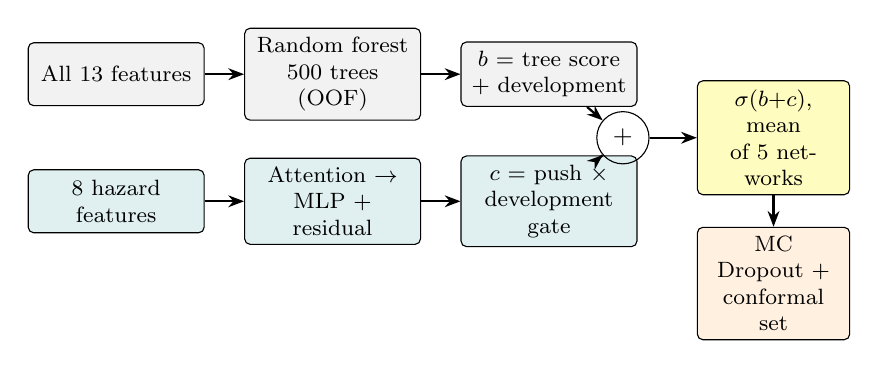
\begin{tikzpicture}[node distance=3.5mm and 5mm,
  box/.style={draw, rounded corners=2pt, align=center, font=\footnotesize, minimum height=8mm, text width=20mm, fill=#1},
  box/.default=white, arr/.style={-{Stealth[length=2mm]}, thick}]
\node[box=gray!10] (all) {All 13 features};
\node[box=gray!10, right=of all] (rf) {Random forest\\500 trees (OOF)};
\node[box=gray!10, right=of rf] (b) {$b$ = tree score\\+ development};
\node[box=teal!12, below=8mm of all] (haz) {8 hazard features};
\node[box=teal!12, right=of haz] (att) {Attention $\rightarrow$\\MLP + residual};
\node[box=teal!12, right=of att] (c) {$c$ = push $\times$\\development gate};
\node[draw, circle, font=\small, right=6mm of $(b)!0.5!(c)$] (plus) {$+$};
\node[box=yellow!25, right=6mm of plus, text width=17mm] (out) {$\sigma(b{+}c)$, mean\\of 5 networks};
\node[box=orange!12, below=4mm of out, text width=17mm] (unc) {MC Dropout +\\conformal set};
\draw[arr] (all) -- (rf); \draw[arr] (rf) -- (b); \draw[arr] (haz) -- (att); \draw[arr] (att) -- (c);
\draw[arr] (b) -- (plus); \draw[arr] (c) -- (plus); \draw[arr] (plus) -- (out); \draw[arr] (out) -- (unc);
\end{tikzpicture}}
\caption{B-ACPN. The deep stage starts from the random-forest score and learns a development term and a development-gated climate push.}
\label{fig:model}
\end{figure}

\subsection{Training}
Each network minimises the class-weighted binary cross-entropy
\par\noindent\begin{minipage}{\columnwidth}
\begin{equation}
\mathcal{L} = -\frac{1}{n}\sum_{i} \omega_{y_i}\big[y_i\log \hat p_i + (1-y_i)\log(1-\hat p_i)\big]
\end{equation}
\begin{symlist}
\item[$\mathcal{L}$] training loss (class-weighted binary cross-entropy);
\item[$n$] number of training districts;
\item[$y_i$] true class of district $i$ (1 = High, 0 = Low vulnerability);
\item[$\omega_{y_i}$] class weight, $0.5$ divided by the share of class $y_i$ in the training set;
\item[$\hat p_i$] predicted probability of high vulnerability for district $i$.
\end{symlist}
\end{minipage}\par

The loss is minimised with AdamW (learning rate $3\times10^{-3}$, weight decay $10^{-3}$, batch 64) for at most 300 epochs, stopping after 30 epochs without improvement on a stratified 15\% validation split. Features are standardised on the training rows of each fold only. Each network has 780 trainable parameters, and one fold trains in 11.8 s on a CPU. Algorithm~\ref{alg:train} summarises the procedure.

\begin{algorithm}[t]
\caption{Training B-ACPN on one fold}
\label{alg:train}
\begin{algorithmic}[1]
\REQUIRE training districts $\{(\mathbf{x}_i, y_i)\}$
\STATE standardise features with training-fold statistics
\FOR{each of 5 inner folds $k$}
  \STATE fit a random forest on the other folds; set $s_i$ for districts in fold $k$
\ENDFOR
\STATE refit the forest on all training districts (used for test scores)
\FOR{$m = 1$ \TO $5$}
  \STATE train deep stage $m$ on $(\mathbf{x}_i, s_i, y_i)$ with early stopping
\ENDFOR
\STATE centre the climate push on the training districts
\STATE calibrate the conformal threshold $\hat q$ on the validation split
\RETURN forest, five deep stages, $\hat q$
\end{algorithmic}
\end{algorithm}

\subsection{Uncertainty}
For each district we run the deep stages 50 times with dropout active and report the standard deviation of the climate push. For classification we use split conformal prediction with nonconformity score $1-\hat p_{y}$: with $\hat q$ the $\lceil (n+1)(1-\alpha)\rceil/n$ empirical quantile of the calibration scores and $\alpha = 0.1$, the prediction set is $\{y : 1-\hat p_y(\mathbf{x}) \le \hat q\}$. Averaged over the folds, the sets cover the true class for 92.9\% of test districts (target 90\%) with an average size of 1.51.

\section{Experiments and Results}
\subsection{Protocol}
All six models use the same splits: repeated stratified five-fold cross-validation with five repeats (25 train/test splits, seed 42) and leave-one-state-out (LOSO) over the 21 states. The five existing models are logistic regression, a random forest (200 trees), gradient-boosted trees (100 iterations, depth 3) and a linear SVM, all trained with Spark MLlib, and a standard multilayer perceptron (13--64--32--16--1) trained with the same loop as B-ACPN. We report means over the 25 folds. Because repeated folds share training data, we compare models with the corrected resampled $t$-test of Nadeau and Bengio \cite{nadeau2003}, which inflates the variance of the paired differences to
\par\noindent\begin{minipage}{\columnwidth}
\begin{equation}
\hat\sigma^2_{c} = \Big(\frac{1}{J} + \frac{n_{\text{test}}}{n_{\text{train}}}\Big)\hat\sigma^2,\qquad J = 25,
\end{equation}
\begin{symlist}
\item[$\hat\sigma^2$] sample variance of the 25 paired per-fold ROC-AUC differences;
\item[$\hat\sigma^2_{c}$] corrected variance used for the $t$-statistic;
\item[$J$] number of train/test splits (folds);
\item[$\frac{n_{\text{test}}}{n_{\text{train}}}$] ratio of test to training districts ($1/4$ for five-fold CV).
\end{symlist}
\end{minipage}\par

We use the same correction for 95\% confidence intervals.

\subsection{Comparison with existing models}
Table~\ref{tab:cmp} gives the main comparison. B-ACPN has the highest ROC-AUC, balanced accuracy, accuracy, F1 and LOSO AUC. Its lead over gradient-boosted trees is smaller than one standard deviation and not significant (p = 0.55), so we regard the two as comparable; against the other four models the difference is significant at the 5\% level. Fig.~\ref{fig:roc} shows the pooled ROC and precision--recall curves.

\begin{table*}[t]
\centering
\caption{Comparison with existing models (mean over 25 folds)}
\label{tab:cmp}
\footnotesize
\setlength{\tabcolsep}{3.5pt}
\begin{tabular}{lcccccc}
\toprule
Model & ROC-AUC & Bal. acc. & Acc. & F1 & LOSO & $p$ \\
\midrule
\textbf{B-ACPN (ours)} & 0.820$\pm$0.035 & 0.739 & 0.738 & 0.728 & 0.717 & -- \\
Gradient-boosted trees & 0.811$\pm$0.034 & 0.726 & 0.725 & 0.724 & 0.698 & 0.550 \\
Random forest & 0.804$\pm$0.036 & 0.715 & 0.715 & 0.708 & 0.706 & 0.042 \\
Standard MLP & 0.784$\pm$0.037 & 0.699 & 0.699 & 0.692 & 0.710 & 0.019 \\
Linear SVM & 0.755$\pm$0.039 & 0.696 & 0.696 & 0.708 & 0.691 & 0.006 \\
Logistic regression & 0.747$\pm$0.042 & 0.691 & 0.692 & 0.701 & 0.661 & 0.004 \\
\bottomrule
\end{tabular}
\end{table*}

\begin{table*}[t]
\centering
\caption{Further classification metrics ($\downarrow$ = lower is better)}
\label{tab:detail}
\footnotesize
\setlength{\tabcolsep}{3.5pt}
\begin{tabular}{lcccccccccc}
\toprule
Model & Prec. & Rec. & Spec. & MCC & $\kappa$ & PR-AUC & LogL$\downarrow$ & Brier$\downarrow$ & ECE$\downarrow$ & RMSE$\downarrow$ \\
\midrule
B-ACPN & 0.765 & 0.700 & 0.778 & 0.482 & 0.477 & 0.844 & 0.516 & 0.174 & 0.108 & 0.417 \\
GBT & 0.736 & 0.718 & 0.733 & 0.454 & 0.451 & 0.826 & 0.570 & 0.188 & 0.131 & 0.433 \\
RF & 0.735 & 0.689 & 0.742 & 0.434 & 0.430 & 0.830 & 0.539 & 0.182 & 0.095 & 0.427 \\
MLP & 0.719 & 0.674 & 0.724 & 0.404 & 0.398 & 0.809 & 0.579 & 0.194 & 0.114 & 0.440 \\
SVM & 0.689 & 0.733 & 0.659 & 0.396 & 0.392 & 0.751 & n/a & n/a & n/a & n/a \\
LR & 0.688 & 0.718 & 0.665 & 0.386 & 0.383 & 0.746 & 0.611 & 0.206 & 0.101 & 0.454 \\
\bottomrule
\end{tabular}
\end{table*}

Table~\ref{tab:detail} lists further metrics. B-ACPN is best on precision, specificity, MCC, Cohen's kappa, PR-AUC, log loss, Brier score and RMSE of the predicted probability. It is not best on recall, where the linear SVM is higher, or on expected calibration error, where the random forest is lower: B-ACPN is more careful about calling a district highly vulnerable, which gives fewer false alarms at the cost of some missed districts.

\begin{figure}[t]
\centering
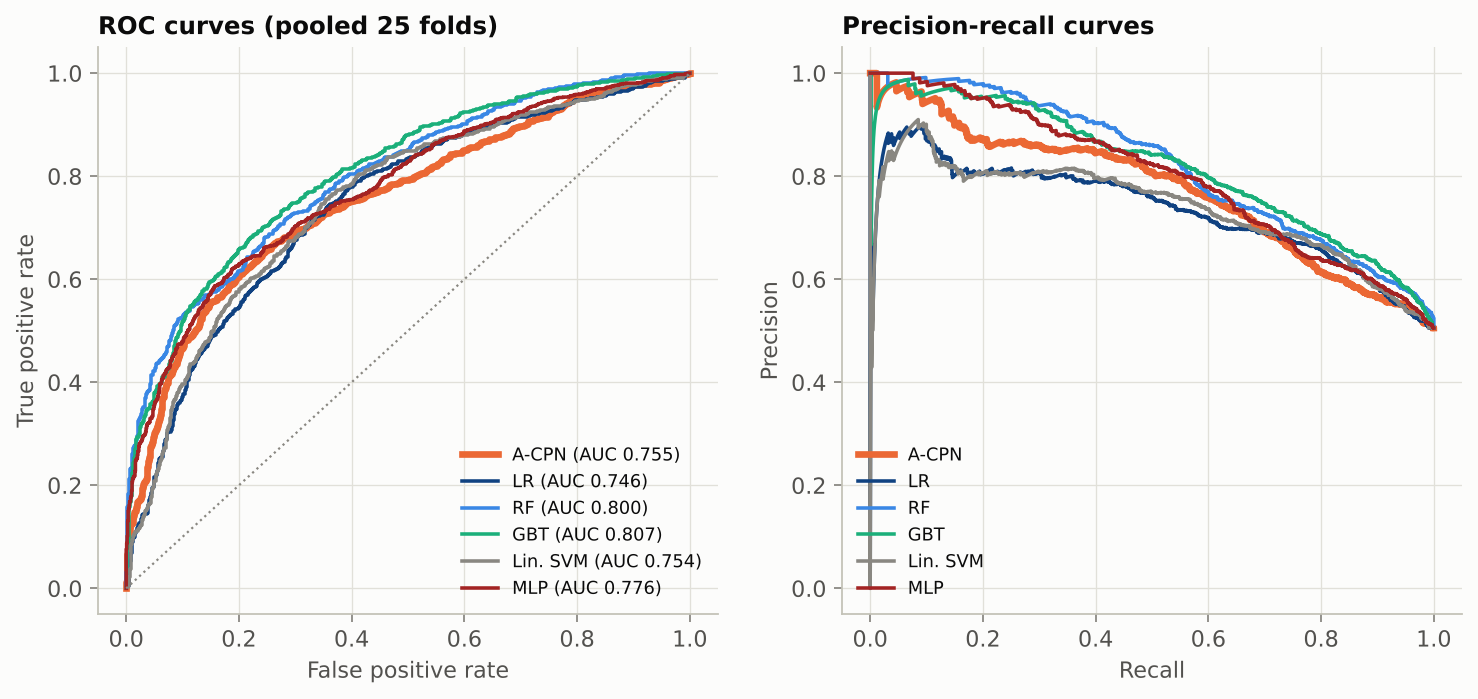
\includegraphics[width=\columnwidth]{roc_curves.png}
\caption{ROC (left) and precision--recall (right) curves of the six models, pooled over the 25 test folds.}
\label{fig:roc}
\end{figure}

\subsection{Effect of preprocessing}
To measure what preprocessing contributes, every model was also trained on the raw, unscaled features with the same folds (Table~\ref{tab:ba}). B-ACPN improves on all reported metrics, for example ROC-AUC from 0.806 to 0.820. The MLP gains ROC-AUC but loses accuracy, because after scaling it labels more districts as highly vulnerable. Tree models are insensitive to feature scale, and Spark's logistic regression and linear SVM standardise internally, so their results do not change.

\begin{table}[t]
\centering
\caption{Before $\rightarrow$ after preprocessing (raw vs.\ preprocessed features)}
\label{tab:ba}
\footnotesize
\setlength{\tabcolsep}{3.5pt}
\begin{tabular}{lcccc}
\toprule
Metric & B-ACPN & MLP & RF & LR \\
\midrule
Accuracy & 0.735$\rightarrow$0.738 & 0.711$\rightarrow$0.699 & 0.715$\rightarrow$0.715 & 0.692$\rightarrow$0.692 \\
Precision & 0.760$\rightarrow$0.765 & 0.776$\rightarrow$0.719 & 0.735$\rightarrow$0.735 & 0.688$\rightarrow$0.688 \\
Recall & 0.700$\rightarrow$0.700 & 0.611$\rightarrow$0.674 & 0.689$\rightarrow$0.689 & 0.718$\rightarrow$0.718 \\
F1 & 0.726$\rightarrow$0.728 & 0.678$\rightarrow$0.692 & 0.708$\rightarrow$0.708 & 0.701$\rightarrow$0.701 \\
Specificity & 0.770$\rightarrow$0.778 & 0.813$\rightarrow$0.724 & 0.742$\rightarrow$0.742 & 0.665$\rightarrow$0.665 \\
ROC-AUC & 0.806$\rightarrow$0.820 & 0.759$\rightarrow$0.784 & 0.805$\rightarrow$0.804 & 0.747$\rightarrow$0.747 \\
MCC & 0.474$\rightarrow$0.482 & 0.437$\rightarrow$0.404 & 0.434$\rightarrow$0.434 & 0.386$\rightarrow$0.386 \\
Log loss$\downarrow$ & 0.528$\rightarrow$0.516 & 0.588$\rightarrow$0.579 & 0.539$\rightarrow$0.539 & 0.611$\rightarrow$0.611 \\
RMSE$\downarrow$ & 0.422$\rightarrow$0.417 & 0.445$\rightarrow$0.440 & 0.427$\rightarrow$0.427 & 0.454$\rightarrow$0.454 \\
\bottomrule
\end{tabular}
\end{table}

\subsection{Ablation}
Table~\ref{tab:abl} removes one part of B-ACPN at a time. Removing the tree stage or the ensemble costs about 0.02 ROC-AUC, the largest drops. Removing the climate push, the attention or the gate changes accuracy by less than one standard deviation; these parts are kept because they provide the per-district explanation, not because they add accuracy.

\begin{table}[t]
\centering
\caption{Ablation of B-ACPN (ROC-AUC, 25 folds)}
\label{tab:abl}
\footnotesize
\setlength{\tabcolsep}{3.5pt}
\begin{tabular}{lccc}
\toprule
Variant & ROC-AUC & Change & $p$ \\
\midrule
Full B-ACPN & 0.820 & -- & -- \\
Deep stage only (no tree stage) & 0.800 & -0.019 & 0.50 \\
Tree stage only (no deep stage) & 0.818 & -0.002 & 0.95 \\
Without climate push & 0.816 & -0.004 & 0.88 \\
Without development gate & 0.821 & +0.001 & 0.96 \\
Without feature attention & 0.817 & -0.003 & 0.93 \\
Single network (no ensemble) & 0.801 & -0.018 & 0.58 \\
\bottomrule
\end{tabular}
\end{table}

\subsection{What the climate push explains}
Fig.~\ref{fig:push} and Table~\ref{tab:push} show the out-of-fold climate push per group. Developed but vulnerable districts (anomaly A) have a positive mean push of +0.09, against -0.10 for developed districts that are not vulnerable (p = $1.6\times10^{-5}$). Less developed but resilient districts (anomaly B) have a negative push of -0.17, against +0.13 for the expected group (p = $4.5\times10^{-7}$). The raw data agree: anomaly A districts have about twice as many tropical nights as expected developed districts (91 vs 45 per year, p = 0.001). Attention gives heavy-rain days the largest mean weight. The Spark climate regimes, found without the model, also differ in push (+0.05 for the larger regime and -0.24 for the smaller one), which supports that the push follows real climate patterns. At the regression level, adding the eight hazards to development raises the explained variance of the index from 0.127 to 0.334.

\begin{figure}[t]
\centering
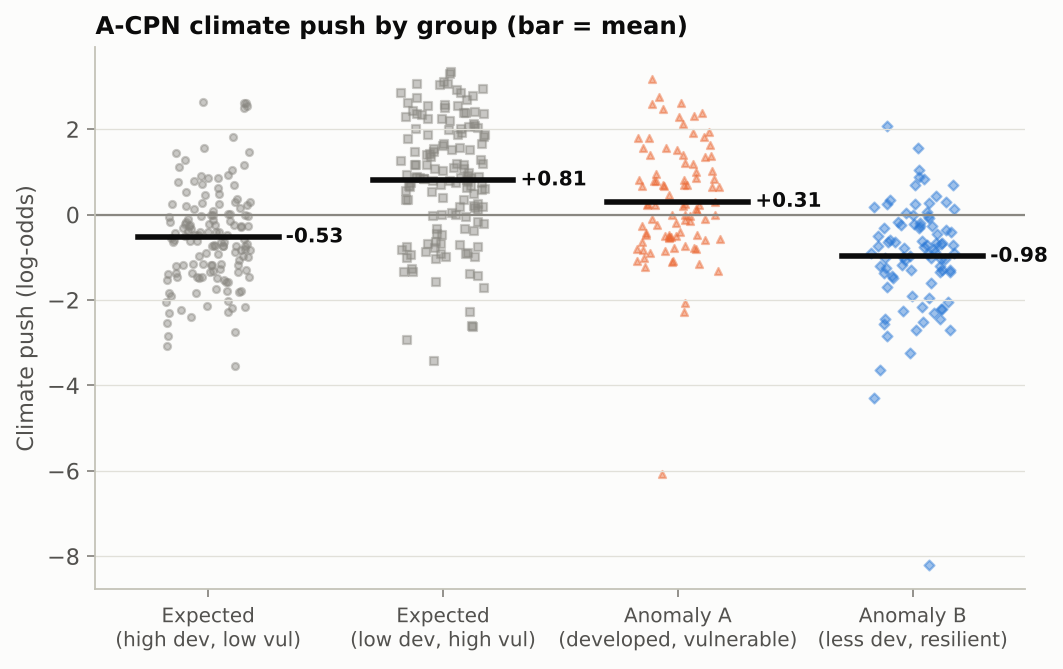
\includegraphics[width=0.92\columnwidth]{climate_push_by_quadrant.png}
\caption{Out-of-fold climate push of every district by group; bars mark group means.}
\label{fig:push}
\end{figure}

\begin{table}[t]
\centering
\caption{Mean climate push by group}
\label{tab:push}
\footnotesize
\setlength{\tabcolsep}{3.5pt}
\begin{tabular}{lccc}
\toprule
Group & $n$ & Push & Push $>$ 0 \\
\midrule
Developed, low vul. (expected) & 143 & -0.10 & 45\% \\
Less developed, high vul. (expected) & 145 & +0.13 & 86\% \\
Anomaly A: developed, vulnerable & 92 & +0.09 & 82\% \\
Anomaly B: less developed, resilient & 89 & -0.17 & 46\% \\
\bottomrule
\end{tabular}
\end{table}

\subsection{Pipeline scaling}
On the single node, MapReduce took 55, 140 and 333 s for 1, 10 and 30 years of input (two runs each). Runtime grows almost linearly with input, while throughput rises from about 4,300 to 21,000 records per second as the fixed job start-up cost is shared over more data.

\section{Discussion}
Three lessons stand out. First, on 469 districts a tree ensemble is a hard baseline, and the network was most useful as a correction on top of it rather than as a replacement; design choices were compared with an inner cross-validation inside the training folds, so the test folds were not used to pick the model. Second, the explanation is not free accuracy: the climate push, attention and gate are kept for interpretability, and the ablation shows that honestly. Third, the Big Data pipeline earns its place through repeatability and checks rather than speed on one machine: each job has an independent pandas check, and the same scripts run on a real cluster.

The work has clear limits. Development comes from Census 2011 while the index is from 2021. Temperature is on a coarse 1\textdegree{} grid. Only five development variables survive without imputation, and 469 districts in 21 states give fold-to-fold standard deviations of about 0.035 ROC-AUC. Hadoop ran on a single node, so no multi-machine speed-up is claimed. The advantage of B-ACPN over gradient-boosted trees is not statistically significant.

\section{Conclusion and Future Work}
We combined a Hadoop pipeline over 30 years of daily IMD climate data with a hybrid model, B-ACPN, to explain why development does not always predict climate resilience in Indian districts. B-ACPN matches or exceeds five existing models on every main metric and, unlike them, assigns each district a climate push with uncertainty, which shows that climate explains much of why developed districts remain vulnerable. Future work will extend HDFS to the full 1901--2024 rainfall record, tune B-ACPN further, compare our district explanations with national vulnerability rankings \cite{ceew2021,dst2020}, and move the pipeline to a multi-node cluster.

\begin{thebibliography}{00}
\bibitem{ceew2021} A. Mohanty and S. Wadhawan, ``Mapping India's climate vulnerability: A district-level assessment,'' Council on Energy, Environment and Water (CEEW), New Delhi, 2021.
\bibitem{dst2020} Department of Science and Technology, Government of India, ``Climate vulnerability assessment for adaptation planning in India using a common framework,'' New Delhi, 2020.
\bibitem{ipcc2022} IPCC, \emph{Climate Change 2022: Impacts, Adaptation and Vulnerability}. Contribution of Working Group II to the Sixth Assessment Report. Cambridge, U.K.: Cambridge Univ. Press, 2022.
\bibitem{pai2014} D. S. Pai, L. Sridhar, M. Rajeevan, O. P. Sreejith, N. S. Satbhai, and B. Mukhopadhyay, ``Development of a new high spatial resolution (0.25\textdegree{} $\times$ 0.25\textdegree{}) long period (1901--2010) daily gridded rainfall data set over India and its comparison with existing data sets over the region,'' \emph{MAUSAM}, vol. 65, no. 1, pp. 1--18, 2014.
\bibitem{srivastava2009} A. K. Srivastava, M. Rajeevan, and S. R. Kshirsagar, ``Development of a high resolution daily gridded temperature data set (1969--2005) for the Indian region,'' \emph{Atmospheric Science Letters}, vol. 10, no. 4, pp. 249--254, 2009.
\bibitem{shvachko2010} K. Shvachko, H. Kuang, S. Radia, and R. Chansler, ``The Hadoop distributed file system,'' in \emph{Proc. IEEE 26th Symp. Mass Storage Systems and Technologies (MSST)}, 2010, pp. 1--10.
\bibitem{dean2008} J. Dean and S. Ghemawat, ``MapReduce: Simplified data processing on large clusters,'' \emph{Commun. ACM}, vol. 51, no. 1, pp. 107--113, 2008.
\bibitem{vavilapalli2013} V. K. Vavilapalli \emph{et al.}, ``Apache Hadoop YARN: Yet another resource negotiator,'' in \emph{Proc. 4th ACM Symp. Cloud Computing (SoCC)}, 2013, pp. 1--16.
\bibitem{thusoo2009} A. Thusoo \emph{et al.}, ``Hive: A warehousing solution over a map-reduce framework,'' \emph{Proc. VLDB Endowment}, vol. 2, no. 2, pp. 1626--1629, 2009.
\bibitem{zaharia2016} M. Zaharia \emph{et al.}, ``Apache Spark: A unified engine for big data processing,'' \emph{Commun. ACM}, vol. 59, no. 11, pp. 56--65, 2016.
\bibitem{meng2016} X. Meng \emph{et al.}, ``MLlib: Machine learning in Apache Spark,'' \emph{J. Mach. Learn. Res.}, vol. 17, no. 34, pp. 1--7, 2016.
\bibitem{breiman2001} L. Breiman, ``Random forests,'' \emph{Machine Learning}, vol. 45, no. 1, pp. 5--32, 2001.
\bibitem{friedman2001} J. H. Friedman, ``Greedy function approximation: A gradient boosting machine,'' \emph{Ann. Statist.}, vol. 29, no. 5, pp. 1189--1232, 2001.
\bibitem{grinsztajn2022} L. Grinsztajn, E. Oyallon, and G. Varoquaux, ``Why do tree-based models still outperform deep learning on typical tabular data?'' in \emph{Advances in Neural Information Processing Systems (Datasets and Benchmarks Track)}, vol. 35, 2022.
\bibitem{arik2021} S. \"{O}. Ar{\i}k and T. Pfister, ``TabNet: Attentive interpretable tabular learning,'' in \emph{Proc. AAAI Conf. Artificial Intelligence}, vol. 35, no. 8, 2021, pp. 6679--6687.
\bibitem{wolpert1992} D. H. Wolpert, ``Stacked generalization,'' \emph{Neural Networks}, vol. 5, no. 2, pp. 241--259, 1992.
\bibitem{he2016} K. He, X. Zhang, S. Ren, and J. Sun, ``Deep residual learning for image recognition,'' in \emph{Proc. IEEE Conf. Computer Vision and Pattern Recognition (CVPR)}, 2016, pp. 770--778.
\bibitem{gal2016} Y. Gal and Z. Ghahramani, ``Dropout as a Bayesian approximation: Representing model uncertainty in deep learning,'' in \emph{Proc. 33rd Int. Conf. Machine Learning (ICML)}, 2016, pp. 1050--1059.
\bibitem{angelopoulos2021} A. N. Angelopoulos and S. Bates, ``A gentle introduction to conformal prediction and distribution-free uncertainty quantification,'' arXiv:2107.07511, 2021.
\bibitem{nadeau2003} C. Nadeau and Y. Bengio, ``Inference for the generalization error,'' \emph{Machine Learning}, vol. 52, no. 3, pp. 239--281, 2003.
\bibitem{rousseeuw1987} P. J. Rousseeuw, ``Silhouettes: A graphical aid to the interpretation and validation of cluster analysis,'' \emph{J. Comput. Appl. Math.}, vol. 20, pp. 53--65, 1987.
\end{thebibliography}

\end{document}
